% DPF 09 talk on strangeness in nucleon

\documentclass[10pt]{beamer}
\usefonttheme{professionalfonts} % using non standard fonts for beamer
\usefonttheme{serif} % default family is serif
\usepackage{amsmath}
\usepackage{ulem}
\usepackage{array}
\usepackage{mathtools}
%\documentclass[12pt]{beamerthemeSam.sty}
\usepackage{epsf}
%\usepackage{pstricks}
%\usepackage[orientation=portrait,size=A4]{beamerposter}
\geometry{paperwidth=160mm,paperheight=120mm}
%DT favorite definitions
\def\LL{\left\langle}	% left angle bracket
\def\RR{\right\rangle}	% right angle bracket
\def\LP{\left(}		% left parenthesis
\def\RP{\right)}	% right parenthesis
\def\LB{\left\{}	% left curly bracket
\def\RB{\right\}}	% right curly bracket
\def\PAR#1#2{ {{\partial #1}\over{\partial #2}} }
\def\PARTWO#1#2{ {{\partial^2 #1}\over{\partial #2}^2} }
\def\PARTWOMIX#1#2#3{ {{\partial^2 #1}\over{\partial #2 \partial #3}} }

\def\rightpartial{{\overrightarrow\partial}}
\def\leftpartial{{\overleftarrow\partial}}
\def\diffpartial{\buildrel\leftrightarrow\over\partial}

\def\BI{\begin{itemize}}
\def\EI{\end{itemize}}
\def\BE{\begin{displaymath}}
\def\EE{\end{displaymath}}
\def\BEA{\begin{eqnarray*}}
\def\EEA{\end{eqnarray*}}
\def\BNEA{\begin{eqnarray}}
\def\ENEA{\end{eqnarray}}
\def\EL{\nonumber\\}
\def\BS{\bigskip}
\def\BC{\begin{center}}
\def\EC{\end{center}}
\def\BCC{\begin{columns}}
\def\ECC{\end{columns}}
\def\HC{\column{0.5\textwidth}}

\newcommand{\etal}{{\it et al.}}
\newcommand{\gbeta}{6/g^2}
\newcommand{\la}[1]{\label{#1}}
\newcommand{\ie}{{\em i.e.\ }}
\newcommand{\eg}{{\em e.\,g.\ }}
\newcommand{\cf}{cf.\ }
\newcommand{\etc}{etc.\ }
\newcommand{\atantwo}{{\rm atan2}}
\newcommand{\Tr}{{\rm Tr}}
\newcommand{\dt}{\Delta t}
\newcommand{\op}{{\cal O}}
\newcommand{\msbar}{{\overline{\rm MS}}}
\def\chpt{\raise0.4ex\hbox{$\chi$}PT}
\def\schpt{S\raise0.4ex\hbox{$\chi$}PT}
\def\MeV{{\rm Me\!V}}
\def\GeV{{\rm Ge\!V}}

%AB: my color definitions
%\definecolor{mygarnet}{rgb}{0.445,0.184,0.215}
%\definecolor{mygold}{rgb}{0.848,0.848,0.098}
%\definecolor{myg2g}{rgb}{0.647,0.316,0.157}
\definecolor{abtitlecolor}{rgb}{0.0,0.255,0.494}
\definecolor{absecondarycolor}{rgb}{0.0,0.416,0.804}
\definecolor{abprimarycolor}{rgb}{1.0,0.686,0.0}
\definecolor{Red}           {cmyk}{0,1,1,0}
\definecolor{Grey}           {cmyk}{.7,.7,.7,0}
\definecolor{Lg}           {cmyk}{.4,.4,.4,0}
\definecolor{Blue}          {cmyk}{1,1,0,0}
\definecolor{Green}         {cmyk}{1,0,1,0}
\definecolor{Brown}         {cmyk}{0,0.81,1,0.60}
\definecolor{Black}         {cmyk}{0,0,0,1}
\definecolor{A}{rgb}{0.8,0.0,0.0}
\definecolor{B}{rgb}{0.0,0.6,0.0}
\definecolor{C}{rgb}{0.6,0.6,0.0}
\definecolor{D}{rgb}{0.0,0.0,0.5}
\definecolor{E}{rgb}{0.4,0.4,0.4}


\usetheme{Madrid}


%AB: redefinition of beamer colors
%\setbeamercolor{palette tertiary}{fg=white,bg=mygarnet}
%\setbeamercolor{palette secondary}{fg=white,bg=myg2g}
%\setbeamercolor{palette primary}{fg=black,bg=mygold}
\setbeamercolor{title}{fg=abtitlecolor}
\setbeamercolor{frametitle}{fg=abtitlecolor}
\setbeamercolor{palette tertiary}{fg=white,bg=abtitlecolor}
\setbeamercolor{palette secondary}{fg=white,bg=absecondarycolor}
\setbeamercolor{palette primary}{fg=black,bg=abprimarycolor}
\setbeamercolor{structure}{fg=abtitlecolor}

\setbeamerfont{section in toc}{series=\bfseries}

%AB: remove navigation icons
\beamertemplatenavigationsymbolsempty
\title{
  \textbf {Moment of inertia}\\
%\centerline{}
%\centering
%\vspace{-0.0in}
%\includegraphics[width=0.3\textwidth]{propvalues_0093.pdf}
%\vspace{-0.3in}\\
%\label{intrograph}
}

\author[W. Freeman] {Physics 211\\Syracuse University, Physics 211 Spring 2017\\Walter Freeman}

\date{\today}

\begin{document}

\frame{\titlepage}

\frame{\frametitle{\textbf{Announcements}}
\large
\BI
\item Physics practice this Wednesday: setting up rotation problems. 7:30-9:30
in Stolkin,
partial solutions to HW7 will be discussed
\item HW7 will be posted today
\item No office hours this Friday (I'll be guest teaching in Arizona)
\item A reminder: if something goes wrong and you can't be in recitation or
turn homework in on time, tell your recitation TA in addition to me
\pause
\item Students who are traveling Easter weekend:
\BI
\item Makeup group exam given Thursday evening, 6PM-7PM or 7PM-8PM
\item You will need to sign up by email, and I'll put you in groups
\item I'll send out info for this tomorrow
\EI
\EI
}

\frame{
\begin{center}
\begin{tabular}{l | l}

 \multicolumn{1}{c|}{\Large Translation} & \multicolumn{1}{c}{\Large Rotation} \\
 \\
\hline
\hline
 & \\
Position $\vec s$ & Angle $\theta$ \\
Velocity $\vec v$ & Angular velocity $\omega$ \\
Acceleration $\vec a$ & Angular acceleration $\alpha$ \\
 & \\
\hline
\hline
 & \\
Kinematics: $\vec s(t)\frac{1}{2}\vec at^2 + \vec v_0 t + \vec s_0$ & $\theta(t) = \frac{1}{2}\alpha t^2 + \omega_0 t + \theta_0$ \\
 & \\
\hline
\hline

 & \\
Force $\vec F$ & Torque $\tau$ \\
Mass $m$ & Rotational inertia $I$ \\
Newton's second law $\vec F = m \vec a$ & Newton's second law for rotation $\tau = I \alpha$ \\
 & \\

\hline
\hline

 & \\
Kinetic energy $KE=\frac{1}{2}mv^2$ & Kinetic energy $KE=\frac{1}{2}I\omega^2$ \\
Work $W = \vec F \cdot \Delta \vec s$ & Work $W = \tau \Delta \theta$ \\
Power $P = \vec F \cdot \vec v$ & Power $P = \tau \omega$ \\
 & \\

\hline
\hline

 & \\
Momentum $\vec p = m \vec v$ & Angular momentum $L = I\omega$\\
 & \\

\hline
\end{tabular}
\end{center}
}

\frame{\frametitle{\textbf Last time}

\Large

Calculating torque:

$$\tau = F_\perp r = F r_\perp = Fr \sin \theta$$

\BI
\item Draw an extended force diagram
\item Label all forces -- both where they act and what they are
\item Write an expression for the torque applied by each
\item Counterclockwise torques are positive; clockwise torques are negative.
\EI

If $\alpha=0$ (``static equilibrium'', ``dynamic equilibrium''):

\BI
\item This means that the net torque (about {\it any} pivot) is zero
\item Choose a pivot on top of a force whose value you {\color{Red} don't know}
and {\color{Red}don't care} about 
\item \color{Red}Write down $\sum \tau = 0$ and solve
\EI
}

\frame{

\Large
\BC
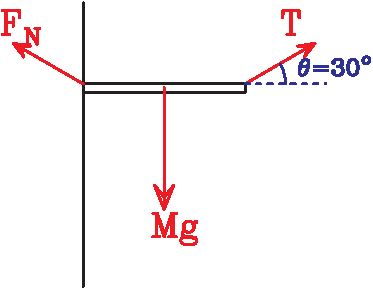
\includegraphics[width=0.5\textwidth]{beam-crop.pdf}

How does the tension $T$ compare to the weight of the beam?

\EC

\BS
\Huge
\BCC
\HC
\color{A}A: $T \leq mg/2$ \\
\color{B}B: $mg/2 < T < mg$ \\
\HC
\color{C}C: $T = mg$ \\
\color{D}D: $mg < T < 2mg$ \\
\ECC
\BC
\color{E}E: $T >=` 2mg$ \\
\EC
}

\frame{\frametitle{\textbf{Beyond equilibrium}}



\begin{center}
\begin{tabular}{l | l}

 \multicolumn{1}{c|}{\Large Translation} & \multicolumn{1}{c}{\Large Rotation} \\
 \\
\hline
\hline
 & \\
Position $\vec s$ & Angle $\theta$ \\
Velocity $\vec v$ & Angular velocity $\omega$ \\
Acceleration $\vec a$ & Angular acceleration $\alpha$ \\
 & \\
\hline
\hline
 & \\
Kinematics: $\vec s(t)\frac{1}{2}\vec at^2 + \vec v_0 t + \vec s_0$ & $\theta(t) = \frac{1}{2}\alpha t^2 + \omega_0 t + \theta_0$ \\
 & \\
\hline
\hline

 & \\
Force $\vec F$ & Torque $\tau$ \\
Mass $m$ & Rotational inertia $I$ \\
Newton's second law $\vec F = m \vec a$ &{\color{Red} Newton's second law for rotation $\tau = I \alpha$} \\
 & \\

\hline
\hline

 & \\
Kinetic energy $KE=\frac{1}{2}mv^2$ & {\color{Red}Kinetic energy $KE=\frac{1}{2}I\omega^2$} \\
Work $W = \vec F \cdot \Delta \vec s$ & Work $W = \tau \Delta \theta$ \\
Power $P = \vec F \cdot \vec v$ & Power $P = \tau \omega$ \\
 & \\

\hline
\hline

 & \\
Momentum $\vec p = m \vec v$ & {\color{Red}Angular momentum $L = I\omega$}\\
 & \\

\hline
\end{tabular}
\end{center}
}

\frame{\frametitle{\textbf{Moment of inertia}}

  \centerline{\Large The analogue of mass is called ``moment of inertia'' (letter $I$)}

  \BI
  \large
\item{More massive things are harder to turn, but that's only part of it}
\item{The mass {\it distribution} matters, too}
\item{The further the mass is from the center, the harder it will be to turn}
\item{The moment of inertia depends on the {\it average squared distance from the center}}
  \EI

  \bigskip\pause

  \centerline{\Large $I=MR^2$}

\bigskip
\bigskip
\bigskip

  \centerline{\large (if all the mass is the same distance from the center)}
  \centerline{\large (our demo rods; hoops; rings; bike wheels)}
}

\frame{\frametitle{\textbf{Moment of inertia: why?}}

\large

To see why $I=M\LL r^2\RR$, let's consider the kinetic energy of a spinning object.

\BS

The kinetic energy of a single ``point mass'' moving in a circle is 
$\frac{1}{2}mv^2 = \frac{1}{2}mr^2\omega^2$, where $r$ is its distance from the 
center.

\BS\pause

Since $KE_{\rm rot}=\frac{1}{2}I\omega^2$, this means $I=mr^2$ for a single point.

\BS\pause

For an extended object, we simply add up the energy of all the moving particles:

$$ I = \int r^2 dm = M \LL r^2 \RR$$

i.e. {\color{Red} the moment of inertia is just the total mass times the 
average squared distance from the axis.}

}

\frame{\frametitle{\textbf{Moment of inertia, other things}}
  \centerline{\Large What about the moment of inertia of other objects?}
  \centerline{\large Requires calculus in general; here are some common ones}
  \centerline{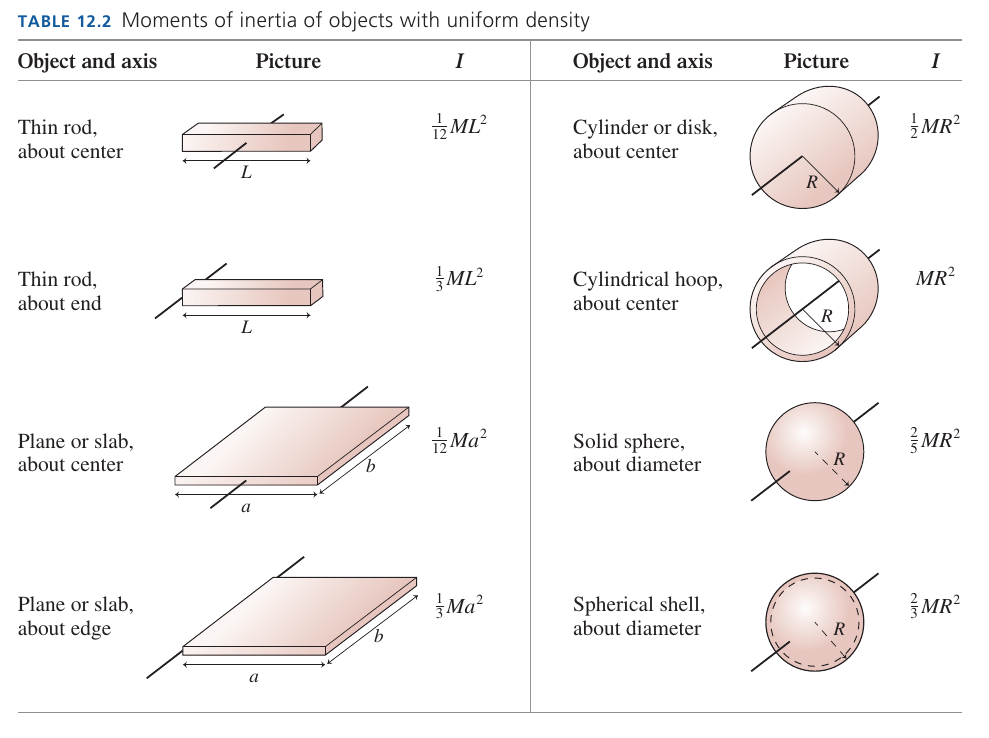
\includegraphics[width=0.7\textwidth]{moment-table.png}}

\BS
\pause
\centerline{In general: $I=\lambda MR^2$}
\centerline{We will always give you $I$ if it's not 1 (i.e. not a ring etc.)}
}

\frame{\frametitle{\textbf{Newton's second law for rotation}}

\Huge

$$\tau = I \alpha$$

\Large

\BC

``Newton's second law for rotation'':

\BS

\large
Torques give things angular acceleration, just like forces make things accelerate.
\EC
}

\frame{

\Large

Which will make the hanging object fall faster?

\BS

\color{A}A: Increasing the diameter of the spool the string is wound around \\
\color{B}B: Decreasing the diameter of the spool the string is wound around \\
\color{C}C: Moving the spinning masses inward \\
\color{D}D: Moving the spinning masses outward \\
\color{E}E: None of the above; it falls at $g$ no matter what
}

\frame{

\Large

What about rotational kinetic energy?

\large

\begin{center}
\begin{tabular}{l | l}

 \multicolumn{1}{c|}{\Large Translation} & \multicolumn{1}{c}{\Large Rotation} \\
 \\
\hline
\hline
 & \\
Position $\vec s$ & Angle $\theta$ \\
Velocity $\vec v$ & Angular velocity $\omega$ \\
Acceleration $\vec a$ & Angular acceleration $\alpha$ \\
 & \\
\hline
\hline
 & \\
Kinematics: $\vec s(t)\frac{1}{2}\vec at^2 + \vec v_0 t + \vec s_0$ & $\theta(t) = \frac{1}{2}\alpha t^2 + \omega_0 t + \theta_0$ \\
 & \\
\hline
\hline

 & \\
Force $\vec F$ & Torque $\tau$ \\
Mass $m$ & Rotational inertia $I$ \\
Newton's second law $\vec F = m \vec a$ & Newton's second law for rotation $\tau = I \alpha$ \\
 & \\

\hline
\hline

 & \\
\color{Blue}
Kinetic energy $KE=\frac{1}{2}mv^2$ & \color{Red}Kinetic energy $KE=\frac{1}{2}I\omega^2$ \\
\color{Blue}
Work $W = \vec F \cdot \Delta \vec s$ & \color{Red}Work $W = \tau \Delta \theta$ \\
\color{Blue}
Power $P = \vec F \cdot \vec v$ & \color{Red}Power $P = \tau \omega$ \\
 & \\

\hline
\hline

 & \\
Momentum $\vec p = m \vec v$ & Angular momentum $L = I\omega$\\
 & \\

\hline
\end{tabular}
\end{center}
}

\frame{
\large

Suppose the pulley were a solid cylinder with mass $M$ and radius $r$.
How fast is the falling mass traveling when it hits the ground if it starts
from a height $h$?

}




\frame{\frametitle{\textbf {Rolling and energy}}

\Large

Which object will reach the bottom of the ramp faster?

\BS

\color{A}A: The wooden one \\
\color{B}B: The one with the mass located near the middle \\
\color{C}C: The one with the mass located near the edge \\
\color{D}D: A tie between A and B \\
\color{E}E: A tie between B and C \\
}





\end{document}
